%!Mode:: "TeX:UTF-8"
\documentclass[a4paper,12pts]{article}

\usepackage[polish]{babel}
\usepackage[utf8]{inputenc}
\usepackage{fontspec}
\setmainfont{Calibri}

\linespread{1.15}

\usepackage{caption}
\captionsetup{%
	font={footnotesize},
	labelfont={bf}
}

\usepackage{anysize}
\usepackage{geometry}

\usepackage{graphicx}

% Plik szablonowy do wykorzystania pózniej - nie zmieniaj go!

\begin{document}
	\thispagestyle{empty}
	\begin{flushleft}
		Wydział Elektrotechniki, Automatyki, Informatyki i Inżynierii Biomedycznej \\
		Informatyka, rok II \\
		Zespół numer 3 \\
		Piotr Kucharski \\
		Dominik Zabłotny \\
		\vspace*{\fill}
		%-----------NUMER CWICZENIA--------%
		{\large \textbf{Sprawozdanie z ćwiczenia nr 35} } \\
		%-----------TEMAT ĆWICZENIA--------%
		Elektroliza		
		\vfill	
		%-----------DATA-------------%
		8 listopada 2017 r.
	\end{flushleft}
	
	\newpage
	
%--------------------------------------------------------------------------------------------------------------
	
	\section{Wstęp}
	
		\subsection{Cel ćwiczenia}
		Celem ćwiczenia jest wyznaczenie stałej Faradaya oraz równoważnika elektrochemicznego miedzi metodą elektrolizy.
	
	%----------------------------------------------------------------------------------------------------------
	
		\subsection{Wprowadzenie teoretyczne}
	
			\subsubsection{Dysocjacja elektrolityczna}
			Proces rozpadu cząstek związków chemicznych na jony pod wpływem rozpuszczalnika nazywamy dysocjacją elektrolityczną. Zjawisku temu podlegają związki z wiązaniami jonowymi oraz bardzo silnie spolaryzowane kowalencyjnie. Jest to proces odwracalny, wiele związków ulega autodysocjacji w stanie ciekłym i gazowym (np. woda).
			
			\subsubsection{Elektroliza}
			Procesy zmiany struktury chemicznej substancji zwykle zachodzące pod wpływem przyłożonego napięcia elektrycznego. Do pojęcia elektrolizy zalicza się wiele zjawisk takich jak dysocjacja elektrolityczna, transport jonów do elektrod, wtórne przemiany jonów na elektrodach i inne. Po przyłożeniu odpowiedniego dla danej substancji napięcia prądu dochodzi do wymuszonej wędrówki jonów do elektrod zanurzonych w  substancji - odpowiednio do katody dążą kationy a do anody dążą aniony. Wynikiem elektrolizy jest zamiana w obojętne elektrycznie związki chemiczne lub pierwiastki. Masa substancji wydzielonej na elektrodzie w wyniku elektrolizy jest wprost proporcjonalna do ładunku przepływającego przez elektrolit (I. prawo Faradaya)
			\begin{equation}
				m = Itk
			\end{equation}
			gdzie $I$ to natężenie prądu, $t$ to czas a $k$ to równoważnik eletrochemiczny.
			
			\subsubsection{Masa molowa}
			Masa jednego mola substancji chemicznej wyrażana jednostką $\frac{\textrm{kg}}{\textrm{mol}}$
			
			\subsubsection{Wartościowość}
			Cecha pierwiastków chemicznych mówiąca o liczbie wiązań chemicznych, którymi pierwiastek lub jon może łączyć się z innymi. Dany pierwiastek może posiadać wiele wartościowości zależnych od stopnia utlenienia.
			
			\subsubsection{Jony}
			Jony to atomy lub grupy atomów połączonych wiązaniami chemicznymi, która ma niedomiar protonów (wówczas nazywamy je anionami) lub nadmiar protonów w stosunku do elektronów (wówczas nazywamy je kationami).
			
			\subsubsection{Katoda}
			Elektroda, przez którą z urządzenia wypływa prąd elektryczny. W urządzeniach elektrycznych katoda jest elektordą ujemną, w źródłach prądu jest elektrodą dodatnią.
			
			\subsubsection{Anoda}
			Elektroda przeciwna do katody, przez nią prąd ,,wpływa" do urządzenia. W odbiornikach jest to elektroda dodatnia a w źródłach prądu ujemna.
			
			\subsubsection{I prawo elektrolizy Faradaya (1834r.)}
			Masa substancji wydzielonej podczas elektrolizy jest proporcjonalna do ładunku, który przepłynął przez elektrolit.
			\begin{equation}
				m = qk = Itk
			\end{equation}
			gdzie $k$ to równoważnik elektrochemiczny, $q$ to ładunek elektryczny, $I$ to natężenie prądu elektrycznego oraz $t$ to czas elektrolizy.
			
			\subsubsection{II prawo elektrolizy Faradaya (1834r.)}
			Ładunek q potrzebny do wydzielenia lub wchłonięcia masy m jest dany zależnością:
			\begin{equation}
				q = \frac{Fmz}{M}
			\end{equation}
			gdzie $F$ to stała Faradaya wrażana jednostką $\frac{\textrm{C}}{\textrm{mol}}$, $z$ to ładunek jonu bez jednostki oraz $M$ to masa molowa jonu wyrażona jednostką $\frac{\textrm{g}}{\textrm{mol}}$
			
			\subsubsection{Stała Faradaya}
			Stała Faradaya wyraża ładunek elektryuczny przypadający na jeden mol eletronów oraz określa się ją wzorem
			\begin{equation}
				F = N_A e
			\end{equation}
			gdzie $N_A$ to stała Avogadra ($N_A \approx 6.022 \cdot 10^{23} \textrm{ mol}^{-1}$) oraz $e$ to ładunek elektronu ($e \approx 1.602 \cdot 10^{-19} \textrm{ C}$). Na podstawie tego wzoru jesteśmy w stanie obliczyć ładunek elementarny dzieląc obie strony równania przez stałą Avogadra.
	
%--------------------------------------------------------------------------------------------------------------

	\section{Wykonanie ćwiczenia}
	Ćwiczenie należy rozpocząć od całkowitego oczyszczenia, wysuszenia, ostudzenia miedzianych blaszek oraz ważenia katody. Uzyskaną masę zapisujemy aby wykorzystać ją do późniejszych obliczeń. Jest to etap konieczny, ponieważ z definicji katody wiemy, że jony wydzielone z elektrolizera ,,wpływają" do katody, stąd masa katody wzrośnie o masę wydzielonych jonów elektrolizera. Następnie należy przygotować układ elektryczny zgodny z schematem przedstawionym na rysunku \ref{schemat_ukladu}. Po podłączeniu blaszek do układu należy zaurzyć zestaw do elektrolizera, włączyć zasilanie oraz skalibrować wartość napięcia oraz oporności na oporniku aby uzyskać natężenie $0.5$ A na amperomierzu. Taki układ pozostawiamy na pół godziny dbając o utrzymanie stałego natężenia w układzie aby elektroliza była jednostajna w czasie. Czas ten jest ważny ze względu na jego późniejsze wykorzystanie w obliczaniu równoważnika elektrochemicznego. Po upływie wyznaczonego czasu ponownie należy przepułkać katodę wodą destylowaną, osuszyć i zważyć ponownie. Uzyskana różnica mas pozwoli na obliczenie stałej Faradaya zgodnie z II prawem elektrolizy Faradaya oraz wartości równoważnika elektrochemicznego zgodnie z I prawem elektrolizy Faradaya.

	
	\begin{figure}[!h]
		\centering
		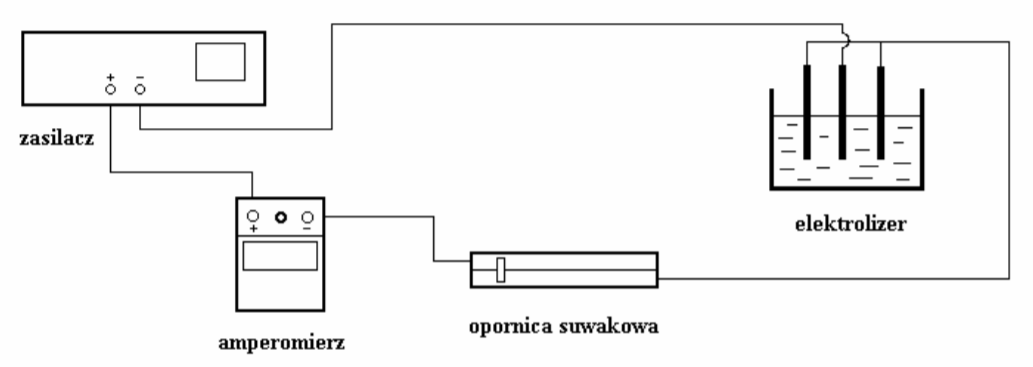
\includegraphics[scale=0.6]{schemat.png}
		\caption{Schemat układu badanego \\ \textit{Źródło: Pracownia Fizyczna WFiIS AGH - ,,Ćwiczenie nr 35: Elektroliza"}}
		\label{schemat_ukladu}
	\end{figure}
	
%--------------------------------------------------------------------------------------------------------------
	
	\section{Opracowanie danych pomiarowych}
	
	\subsection{Wykonane pomiary}
	
	\begin{enumerate}
		\item Czas elektrolizy:
		\begin{equation}
		t = 30 \textrm{ [min]} = 1800 \textrm{ [s]}
		\end{equation}
		
		\item Natężenie prądu:
		\begin{equation}
		I = 0,5 \textrm{ [A]}
		\end{equation}
		
		\item Masa katody przed elektrolizą:
		\begin{equation}
		m_{1} = 61.337 \textrm{ [g]}
		\end{equation}
		
		\item Masa katody po elektrolizie:
		\begin{equation}
		m_{2} = 61.646 \textrm{ [g]}
		\end{equation}
		
		\item Masa wydzielonej miedzi:
		\begin{equation}
		m = m_{2} - m_{1} = 0.309 \textrm{ [g]}
		\end{equation}
	\end{enumerate}
	
	%--------------------------------------------------------------------------------------------------------------
	
	\newpage
	\subsection{Dane określające niepewność przyrządów}
	
	\begin{enumerate}
		\item Klasa amperomierza: 
		$$0.5 \textrm{ [\%]}$$
		\item Używany zakres amperomierza: 
		$$0.75 \textrm{ [A]}$$
		\item Niepewność graniczna wagi (znamionowa): 
		$$\Delta m = 0.001 \textrm{ [g]}$$
		\item Niepewność standardowa wagi: 
		$$u(m) = \frac{\Delta m}{\sqrt{3}} = 0.00057 \textrm{ [g]}$$
	\end{enumerate}
	
	%--------------------------------------------------------------------------------------------------------------
	
	\subsection{Obliczenia}
	
	\begin{enumerate}
		\item Masa miedzi wydzielonej podczas elektrolizy na katodzie:
		$$m = 0.309 \textrm{ [g]}$$
		\item Wartość współczynnika elektrochemicznego miedzi na podstawie przekształconego wzoru (1): 
		$$k = \frac{m}{I \cdot t} = 0.00034 \textrm{ [g/C]}$$
		\item Na podstawie otrzymanej wartości współczynnika elektrochemicznego możemy ze wzoru  obliczyć eksperymentalną wartość stałej Faraday'a:
		$$F = 	
	\end{enumerate}
		
%----------------------------------------------------------------------------------------------------------	
	
	\subsection{Analiza niepewności}
	
%--------------------------------------------------------------------------------------------------------------

	\section{Podsumowanie}

%--------------------------------------------------------------------------------------------------------------
	
	\section{Wnioski}

\end{document}